\documentclass{article}
\usepackage[utf8]{inputenc} 
\usepackage[spanish]{babel}
\usepackage{url} 
\usepackage{enumerate}
\usepackage{graphicx}
\usepackage{float}
\usepackage{colortbl}
\usepackage[colorlinks=true,linkcolor=black,urlcolor=black, citecolor=black]{hyperref}

\begin{document}
\section{Manual de usuario de PrediXaber11}
La aplicación web PrediXaber11 cuenta con 5 opciones diferentes para obtener información de la pagina.
\begin{itemize}
\item \textbf{Inicio:} Esta es la pagina de bienvenida a la aplicación, aquí se encuentra información sobre que cual es el objetivo de esta aplicación web.
\begin{figure}[H]
\begin{centering}
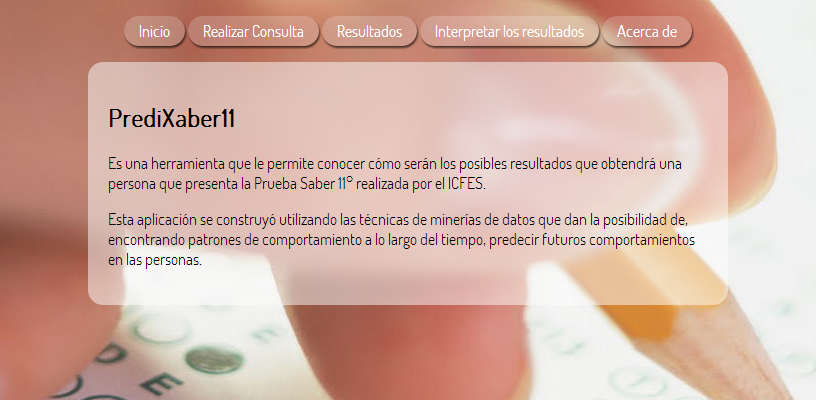
\includegraphics[scale=0.4]{inicio}
\par\end{centering}
\label{fig:figura6}
\end{figure}
\item \textbf{Realizar Consulta:} En esta parte, se debe rellenar el formulario con la información correspondiente a la persona de la cual se quiere saber los posibles resultados en la prueba Saber 11{\ensuremath{^\circ}}
\begin{figure}[H]
\begin{centering}
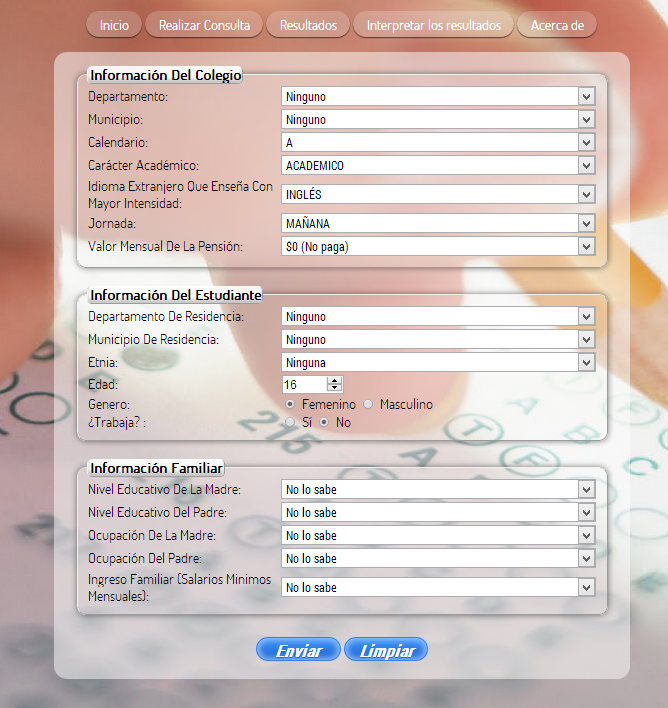
\includegraphics[scale=0.5]{consultar}
\par\end{centering}
\label{fig:figura6}
\end{figure}
Cuando se presione en el botón ``Enviar'', la información sera procesada por la aplicación. En este momento se vera la siguiente imagen, indicando que la información esta siendo procesada.
\begin{figure}[H]
\begin{centering}
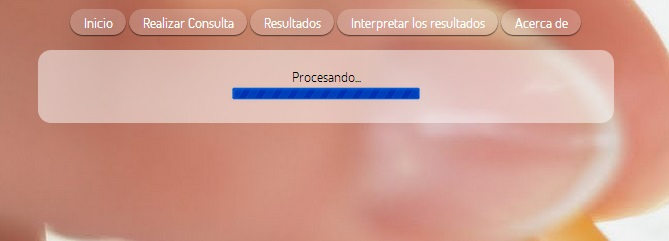
\includegraphics[scale=0.5]{procesando}
\par\end{centering}
\label{fig:figura6}
\end{figure}
\item \textbf{Resultados:} Después de procesar la información, la aplicación retornara una respuesta similar a la mostrada en la siguiente imagen.
\begin{figure}[H]
\begin{centering}
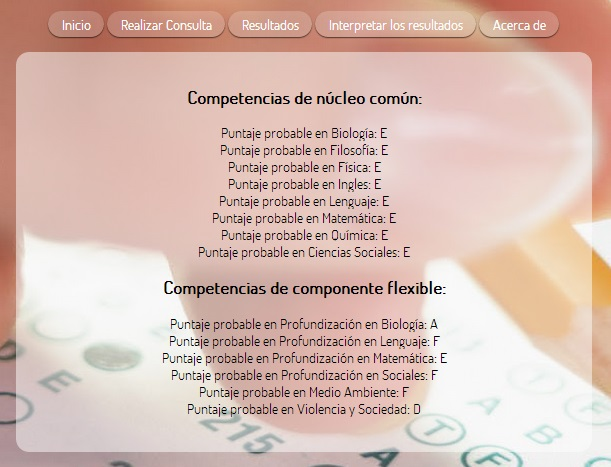
\includegraphics[scale=0.6]{resultados}
\par\end{centering}
\label{fig:figura6}
\end{figure} 
En caso de que se acceda a la opción ``Resultados'' antes de haber realizado alguna consulta, la información mostrada sera la siguiente.
\begin{figure}[H]
\begin{centering}
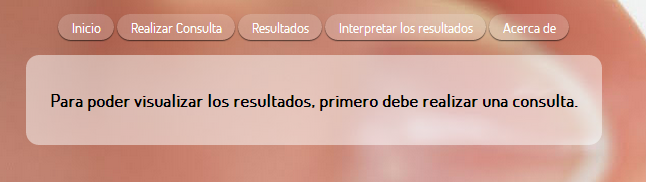
\includegraphics[scale=0.6]{resultado}
\par\end{centering}
\label{fig:figura6}
\end{figure}
\item \textbf{Interpretar los resultados:} En esta sección se podrá observar como se deben interpretar los resultados entregados por la aplicación.
\begin{figure}[H]
\begin{centering}
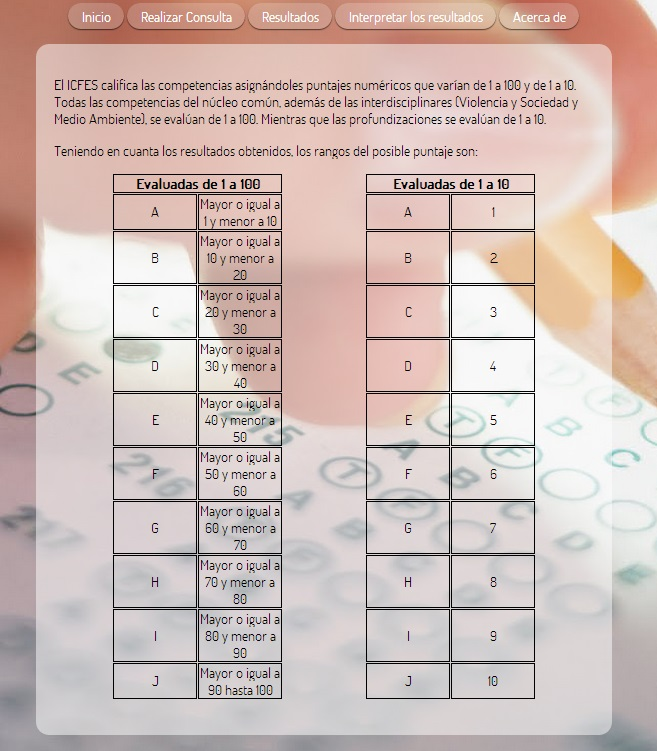
\includegraphics[scale=0.5]{interpretar}
\par\end{centering}
\label{fig:figura6}
\end{figure}
\item \textbf{Acerca de:} En esta sección se podrá encontrar información sobre el desarrollo de la aplicación PrediXaber11.
\begin{figure}[H]
\begin{centering}
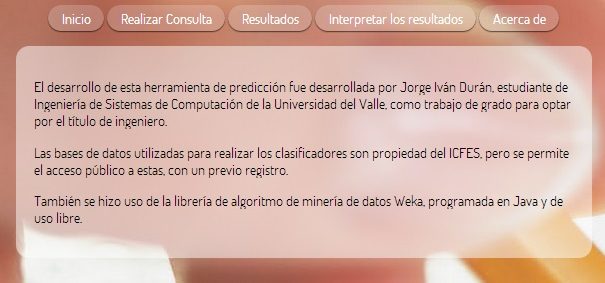
\includegraphics[scale=0.5]{about}
\par\end{centering}
\label{fig:figura6}
\end{figure}
\end{itemize}



\end{document}